\documentclass[./Thesis]{subfiles}


\graphicspath{{./Images/}}

\begin{document}

\chapter{Introduction to the Muon G-2 Experiment}

In the following chapter there will be an explanation of the history of the experiment, why the experiment is being performed, along with the fundamental aspects of GM2.  Furthermore, there will be an explanation of the results from the previous experiment E821 and how this relates to standard model predictions. This gives the fundamental reasoning for performing E989, the current G-2 experiment.

\section{History and Motivation}

The muon anomalous magnetic moment has been measured in a series of experiments at CERN and more recently in the E821 experiment at the Brookhaven National Laboratory. In the first CERN measurements, muons were injected into a 6-m long straight magnet where they followed a drifting spiral path slowly traversing the magnet because of a small gradient introduced in the field. The muons were topped in a polarimeter outside the magnet and the measurement of their net spin precession determined with an uncertainty of 4300 ppm.  The results agreed with the prediction of QED for a structureless particle.\cite{Cern1} The second CERN experiment used a magnetic ring to extend the muon storage time. The muon precession frequency was measured by the number of decayed positrons versus time and observing the precession frequency of the decayed positrons. They were able to determine the value of to an uncertainty of 270 ppm, which agreed with theory only after the three-photon exchange contribution to the sixth-order anomalous magnetic moment were included.\cite{Cern2}  Furthermore, the third CERN experiment also used a magnetic storage ring with a much higher rate and was able to determine the value to within an uncertainty of 10 ppm, which also agreed with theory.\cite{Cern3} The most recent Brookhaven Experiment, E821, followed the same principles as the third CERN experiment but having multiple improvements in the field uniformity and increased storage efficiency. E821 was able to determine to an uncertainty of 0.54 ppm.  Ref.\cite{TDR}

\subsection{Magnetic and Electric Dipole Moments}

The study of magnetic moments started with the development of quantum mechanics.  For fermions it is related to the spin by the Eq.\ref{EQ:MDM}. This is derived from the fact that if there is circular loop of a wire carrying a current $I$ with a cross sectional area $A$, it produces a magnetic moment $\mu$.  The current is given by Eq.\ref{EQ:current} where q is the charge, r is the radius of the loop, and $Q=\pm1$ taking account of the charge. The area is given by Eq.\ref{EQ:area} where v would be the velocity of the particle.

	\begin{equation}\label{EQ:MD}
	\vec{\mu} = I\vec{A} 
	\end{equation}

	\begin{equation}\label{EQ:current}
	I = \frac{Qqv}{2\pi r}
	\end{equation}
	
	\begin{equation}\label{EQ:area}
	A = \pi r^2
	\end{equation}
	
 By plugging in Eq.\ref{EQ:current} and Eq.\ref{EQ:area} into Eq.\ref{EQ:MD}  yields Eq.\ref{EQ:MD1}.

	\begin{equation}\label{EQ:MD1}
	\vec{\mu} = \frac{Qq}{2m}\vec{L}
	\end{equation}

Using the relation of angular momentum $L = mvr$ and knowing the only contribution to angular momentum of a free particle is due only to its spin this gives Eq.\ref{EQ:MD2}.  In the modern interpretation of the Stern Gerlach experiment which observed that the spin is quantized and \ref{EQ:MD2} is off by a factor of 2.\cite{Stern} To correct for this there was added a fudge factor called the g-factor giving \ref{EQ:MDM}.  Although, coming to this conclusion required the discovery of the spin, quantum mechanics, and Thomas' relativistic correction. Where Thomas' correction applies to the spin of an elementary particle and relates the angular velocity of the spin to the angular velocity of the particles motion.

	\begin{equation}\label{EQ:MD2}
	\vec{\mu} = \frac{Qq}{2m}\vec{s}
	\end{equation}


	\begin{equation}\label{EQ:MDM}
	\vec{\mu} = g \frac{Qq}{2m} \vec{s}
	\end{equation}
	
In 1928 Dirac applied special relativity to Schrodinger's equation.  Dirac's relativistic theory predicted that $g=2$.  In 1933 Stern showed that that the g-factor of the proton was approximately 5.5 which proved that the proton was not a pure Dirac particle.\cite{Stern2}  In addition, Alvarez and Bloch discovered the neutron had a large magnetic moment which was not expected.\cite{Bloch}  In 1947, motivated by measurements of the hyperfine structure in hydrogen, Schwinger showed that from a theoretical standpoint this splitting can be accounted for by adding in a term for the electron spin magnetic moment for the lowest radiative correction to the Dirac moment.\cite{Schwinger}

	\begin{equation}
	\frac{\delta\mu}{\mu}  = \frac{1}{2 \pi } \frac{e^2}{\hbar c}
	\end{equation}
	
It has been found useful to break the magnetic dipole moment into two terms as follows with $a$ being the anomalous magnetic moment.  Ref.\cite{TDR}
	
	\begin{equation}
	\mu = (1+a)\frac{e\hbar}{2m}
	\end{equation}
	Where
	\begin{equation}
	a = \frac{g-2}{2}
	\end{equation}
	
	
\subsection{The Muon}

	The muon was first observed in a Wilson cloud chamber by Kunze in 1933.\cite{Cloud} In 1936, Anderson and Neddermeyer reported that the muon is less massive than the proton but more penetrating than the electron.\cite{Nevis} Muon decays through the force $\mu^- \rightarrow e^{-}\nu_{\mu}\overline{\nu}_{e}$. With the muons long lifetime of approximately 2.2 $\mu$s this permits precession measurements of its mass, lifetime, and magnetic moment which makes the muon a good candidate for experiments.\cite{TDR}

\subsection{The Muon Magnetic Moment}

	The muon magnetic moment played an important role in the discover of the generation structure of the standard model.  The muon spin experiment at Nevis Cyclotron witnessed parity violation in muon decays, in addition to showing that $g_\mu$ is consistent with 2.  Later experiments showed that in a magnetic field the muon behaves like a heavy electron.  Ref.\cite{TDR}


\subsection{The Muon Electric Dipole Moment}

	In his relativistic theory Dirac discovered an EDM and like the magnetic dipole moment, the EDM must be in the direction of the spin.  The equation for the Electric dipole moment is given by Eq.\ref{EQ:EDM}.
	
	\begin{equation}\label{EQ:EDM}
		\vec{d} = \eta (\frac{Qe}{2mc}) \vec{s}
	\end{equation}

	Where $\eta$ is dimensionless and analogous to g in Eq. \ref{EQ:MDM}.  An EDM is forbidden by parity and by time reversal which was first pointed out by Landau and Ramsey by examining the Hamiltonian given by Eq.\ref{EQ:Hamiltonian}. \cite{Landau}
	
	\begin{equation}\label{EQ:Hamiltonian}
	H = -\vec{\mu} \cdot \vec{B} - \vec{d} \cdot \vec{E}
	\end{equation}
	
Therefore, searches for a permanent EDM of electrons, neutrons, and atomic nucleus have become an important search for physics beyond the standard model.  Ref.\cite{TDR}

\section{Quick Summary of Experimental Technique}

	In the modern G-2 experiment E989, a polarized beam of muons is produced and injected into a storage ring from the Fermilab accelerator complex.  The magnetic field is a dipole field in the storage ring with vertical focusing being provided by the electrostatic quadrupoles.  There are two frequencies are measured experimentally, the first frequency $\omega_{a}$ is the rate at which the muon polarization turns relative to the momentum of the muon, and the second frequency $\omega_p$ is the value of the magnetic field normalized to the Lamour frequency.
	
	\begin{equation}
	\vec{\omega}_{a} = \vec{\omega}_{S} - \vec{\omega}_{C}
	\end{equation}

Where S denotes the spin and C denotes the cyclotron which the individual terms are given by Eq.\ref{EQ:omegaS} and Eq.\ref{EQ:omegaC}

	\begin{equation}\label{EQ:omegaS}
	\omega_{S} = -g \frac{Qe}{2m} B - (1-\gamma)\frac{Qe}{\gamma m} B
	\end{equation}

	\begin{equation}\label{EQ:omegaC}
	\omega_C = - \frac{Qe}{m\gamma} B
	\end{equation}

It is worth noting that $\omega_a$ depends only on the anomaly $a_\mu$ and depends linearly on the applied magnetic field.  In the presence of an electric field we get \ref{EQ:omegaA}

\begin{equation}\label{EQ:omegaA}
\vec{\omega}_a = -\frac{Qe}{m}[a_{\mu} \vec{B} + (a_{\mu} - (\frac{m}{p})^2) \frac{\vec{\beta} \times \vec{E}}{c}]
\end{equation}


If $p_{magic} = \frac{m}{\sqrt{a_\mu}} \equiv 3.09 \frac{GeV}{c}$ the electric field contribution in Eq. \ref{EQ:omegaA} cancels to the first order which only requires higher order corrections to the term. The factor $a_\mu$ from the two frequencies we use the relation \ref{EQ:amu}.

\begin{equation}\label{EQ:amu}
a_\mu = \frac{\omega_a / \omega_p}{\lambda_{+} - \omega_a / \omega_p}
\end{equation}

The necessary steps in the experiment consist of the following.  Ref. \ref{TDR}


1.	Production of an appropriate pulsed proton beam from accelerator complex.

2.	Production of pions using this proton beam.

3. 	Collection of the polarized muons from pion decay.

4. 	Injection of the muon beam into the storage ring.

5. 	Kicking the muon beam onto stored orbits

6.	Measuring the arrival time and energy of positrons form the muon decays.


\vspace{5mm}

\subsection{Quick Introduction to Muon Beam Dynamics}

	Here is given a quick introduction to the physics of the beam dynamics of a weakly focused betatron which is used in the current E989 experiment.  This section is mainly used to give an introduction to the pitch correction and the radial field correction which will be discussed later in the systematics study. 

	Beam dynamics of the storage ring directly affects the measurement of $a_\mu$ since the detector acceptance for the decay electrons depends on the radial coordinate of the muon at the point where it decays.  Resonances in the storage ring also can cause particle losses which affect the measurement.  Care is taken in the experiment in setting the frequency of the coherent betatron oscillation which lies close to the second harmonic $f_a = \omega_a / 2\pi$.  If $f_{cbo}$ is too close to $2\times f_a$, which is the beat frequency, this complicates the extraction of $f_a$ from the data and can introduce significant systematic uncertainty.  

	A pure quadrupole electric field supplies a linear restoring force in the vertical direction and the combination of the electric field.  The central magnetic field provides a linear restoring force in the radial direction. The G-2 storage ring is a weak focusing ring with the field index given by Eq.\ref{EQ:FieldIndex}.

	\begin{equation}\label{EQ:FieldIndex}
	n =\frac{\kappa R_0}{\beta B_0}
	\end{equation}

	Where $\kappa$ is the electric quadrupole gradient, $B_0$ is the magnetic field strength, $R_0$ is the magic radius, and $\beta$ is the relativistic velocity of the muon beam.  For a ring with a uniform vertical dipole magnetic field and a uniform quadrupole field the horizontal and vertical motion is given by Eq.\ref{EQ:VerticalCBO} and Eq.\ref{EQ:horizontalCBO} respectively.
	
	\begin{equation}
	\label{EQ:VerticalCBO}
	x = x_e +A_x cos(\nu_x \frac{s}{R_0} + \delta_x)
	\end{equation}

	\begin{equation}
	\label{EQ:horizontalCBO}
	y =  A_y cos(\nu_y \frac{s}{R_0} + \delta_y)
	\end{equation}
Where $s$ is the arc length along the trajectory of the ring. The horizontal and vertical tunes are given by Eq.\ref{EQ:verticalTune} and  Eq.\ref{EQ:horizontalTune} respectively.

	\begin{equation}
	\label{EQ:verticalTune}
	\nu_x = \sqrt{1-n}
	\end{equation}

	\begin{equation}
	\label{EQ:horizontalTune}
	\nu_y = \sqrt{n}
	\end{equation}
In E821 there were several tunes used for in the data acquisition $n = 0.137, 0.142, 0.122$. The horizontal and vertical betatron frequencies are given by Eq.\ref{EQ:verticalFreq}  and  Eq.\ref{EQ:horizontalFreq} repectively.

	\begin{equation}
	\label{EQ:verticalFreq}
	f_x = f_c \sqrt{1-n} \equiv 0.929 f_c
	\end{equation}
	
	\begin{equation}
	\label{EQ:horizontalFreq}
	f_y = f_c \sqrt{n} \equiv 0.37f_c
	\end{equation}

Where $f_c$ is the cyclotron frequency and $n=0.137$. The field index also determines the angular acceptance of the ring where the maximum horizontal and vertical angle of the muon momentum are given by Eq.\ref{EQ:verticalAngle} and Eq.\ref{EQ:horizontalAngle} respectively.

	\begin{equation}
	\label{EQ:verticalAngle}
	\theta^{x}_{max} = \frac{x_{max} \sqrt{1-n}}{R_0}
	\end{equation}

	\begin{equation}
	\label{EQ:horizontalAngle}
	\theta^{y}_{max} = \frac{y_{max} \sqrt{n}}{R_0}
	\end{equation}

Where $x_{max} ,y_{max} =  45mm$ which is the radius of the storage ring aperture.

For a ring with discrete quads the focusing strength changes as a function of azimuth and the equation of motion looks like an oscillator where the spring constant constantly changes as a function of azimuth $s$. 

	\begin{equation}
	X(s) = x_e + A \sqrt{\beta(s)} cos(\phi(s)+\delta)
	\end{equation}
	
The presence of the coherent betatron oscillation was first discovered in the E821 experiment from a plot that showed there was in azimuthal variation in $a_\mu$ so this led to a correction factor.

In the simplest case with the absence of an electric field and when the velocity is perpendicular to the magnetic field, the rate at which the spin precesses relative to the momentum is given by Eq.\ref{EQ:omegaA}.
	
	\begin{equation}
	\label{EQ:omegaA}
	\omega_{a} = -a\frac{Qe}{m} B
	\end{equation}

However, in the real experiment not all the muons are at the magic momentum, therefore a precision knowledge of the trajectories required.  To look at this effect we calculate the effect on the electric field due to muon not directly at $\gamma_{magic}$, for the moment neglecting the $\vec{\beta}\cdot\vec{B}$ terms.

	\begin{equation}
	\omega_{a}' = \omega_{a}[1-\beta\frac{E_r}{B_y}(1-\frac{1}{a_\mu \beta^2 \gamma^2})]
	\end{equation}

Where $\omega_{a} = -a \frac{Qe}{m}B$. Now using the fact that $p=\beta\gamma m = p_m + \Delta p$ we get Eq.\ref{EQ:deltaomega}.


\begin{equation}
\label{EQ:deltaomega}
\frac{\Delta \omega_a}{\omega_a} = -2 \frac{\beta E_r}{B_y}(\frac{\Delta P}{P_m})
\end{equation}

Where the fractional change in momentum in Eq.\ref{EQ:deltaomega} can be represented as Eq.\ref{EQ:deltap}

\begin{equation}
\label{EQ:deltap}
\frac{\Delta P}{P_m}=(1-n)\frac{\Delta R}{R_0} = (1-n) \frac{X_e}{R_0}
\end{equation}


Where the $X_e$ is the muons beam equilibrium radius. Then the electric quadrupole field is given by Eq.\ref{EQ:Efield}

\begin{equation}
\label{EQ:Efield}
E = \kappa X = \frac{n\beta B_y}{R_{0}}x
\end{equation}

Therefore we obtain the final result to the change in frequency Eq.\ref{EQ:deltaw}.

\begin{equation}
\label{EQ:deltaw}
\frac{\Delta \omega}{\omega} = -2n(1-n)\beta^2\frac{x x_e}{R_0^2 B_y}
\end{equation}

Therefore, the effect of muons not at the magic momentum is to lower the measured $\omega_a$ frequency.  For a quadrupole focusing field plus a uniform magnetic field the time average of $<x> = x_e$, so the electric field correction is given by Eq.\ref{EQ:EFieldCorrection}. The value $<x_e^2>$ is determined in the fast rotation analysis which will not be covered in this thesis.  In the Brookhaven experiment it was found for a low n that $C_E = 0.47 \pm 0.054 ppm$.

\begin{equation}
\label{EQ:EFieldCorrection}
C_E = \frac{\Delta\omega}{\omega} = -2n(1-n)\beta^2\frac{<x_e^2>}{R_0^2 B_y}
\end{equation}

The betatron oscillations of the muon beam lead to the terms $\vec{\beta}\cdot\vec{B}\neq0$. Since the $\vec{\beta}\cdot\vec{B}$ term is quadratic in the component of $\vec{\beta}$, its contribution to $\vec{\omega_s}$ will not generally average out to zero. The spin precession frequency has a small dependence on the betatron motion of the beam. In addition, it turns out the only significant correction comes from the vertical betatron oscillations which is called the pitch correction. The pitch angle varies harmonically as in Eq.\ref{EQ:betatron}

\begin{equation}
\label{EQ:betatron}
\psi = \psi_0 Cos(\omega_y t)
\end{equation}

Where $\omega_y$ is the vertical betatron frequency. If we set $a_\mu - \frac{1}{\gamma^2-1}=0$ we obtain \ref{EQ:omegaDiff}

\begin{equation}
\label{EQ:omegaDiff}
\vec{\omega}_{diff} = - \frac{Qe}{m}[a_\mu \vec{B} - a_\mu(\frac{\gamma}{\gamma+1})(\vec{\beta}\cdot\vec{B})\vec{\beta}]
\end{equation}

Now if we assume that the pitch angles are small, $\vec{B} = \hat{y} B_y$ , $\beta=\hat{z}\beta_z + \hat{y}\beta_y$ then the difference in frequency is given by Eq.\ref{EQ:oDiff}.

\begin{equation}
\label{EQ:oDiff}
\omega_{ay}' = -\omega_a[1-(\frac{\gamma -1 }{\gamma})\psi^2]
\end{equation}


This then gives the pitch correction found in Eq.\ref{EQ:pitchCorrection}.

\begin{equation}
\label{EQ:pitchCorrection}
C_p = - \frac{<\psi^2>}{2} = - \frac{n}{4}\frac{<y^2>}{R_0^2}
\end{equation}

The result that the pitch correction and the radial field corrections are dependent on the average positions is what makes straw trackers important in E989 since these detectors have the best resolution for position measurements. 

\section{Results from Brookhaven Experiment}
	The Brookhaven based experiment E821 which was completed in 2001 was a successful experiment in its achievements.  As previously mentioned, the experiment was able to measure the precession frequency to approximately 14 times better than what was ever achieved before in the previous CERN experiments. Steady improvements in the theory resulted in a present measurement of $a_\mu$ with an uncertainty of 0.42 ppm.  The E821 experiment was able to reach a field uniformity to $\pm1$ ppm uniformity on average.  The main systematical uncertainties of this experiment were caused from anything that caused the extracted frequency to vary the true fit value.  Uncertainties in the $\omega_a$ measurement mainly consist of gain instability in the detectors, lost muons, spin tracking, coherent betatron oscillations, differential decays, and pitch correction uncertainties.  The main source of uncertainty from the $\omega_p$ measurement consist of errors due to non-uniformity in the magnetic field.  The results for E821 are given in Fig. \ref{fig:E821Results} which show previous measurements and the Standard Model Predictions which shows that there was a discrepancy from standard model values for $a_\mu$ and the Brookhaven National Laboratory experiment measured values up to 3.5 standard deviations. Ref.\cite{TDR}
	
\begin{figure}
\centerline{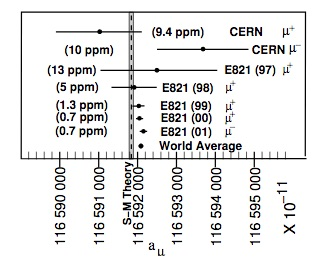
\includegraphics[height=95mm]{E821Result.jpg}}
\caption[$a_\mu$ results after E821]{ Measurement of $a_\mu$ from CERN and BNL E821. The vertical band in the SM value using the hadronic contribution. \cite{TDR}
	}
\label{fig:E821Results}
\end{figure}



\end{document}